\section{Method}
\label{sec:method}

\begin{figure*}[t]
    \centering
    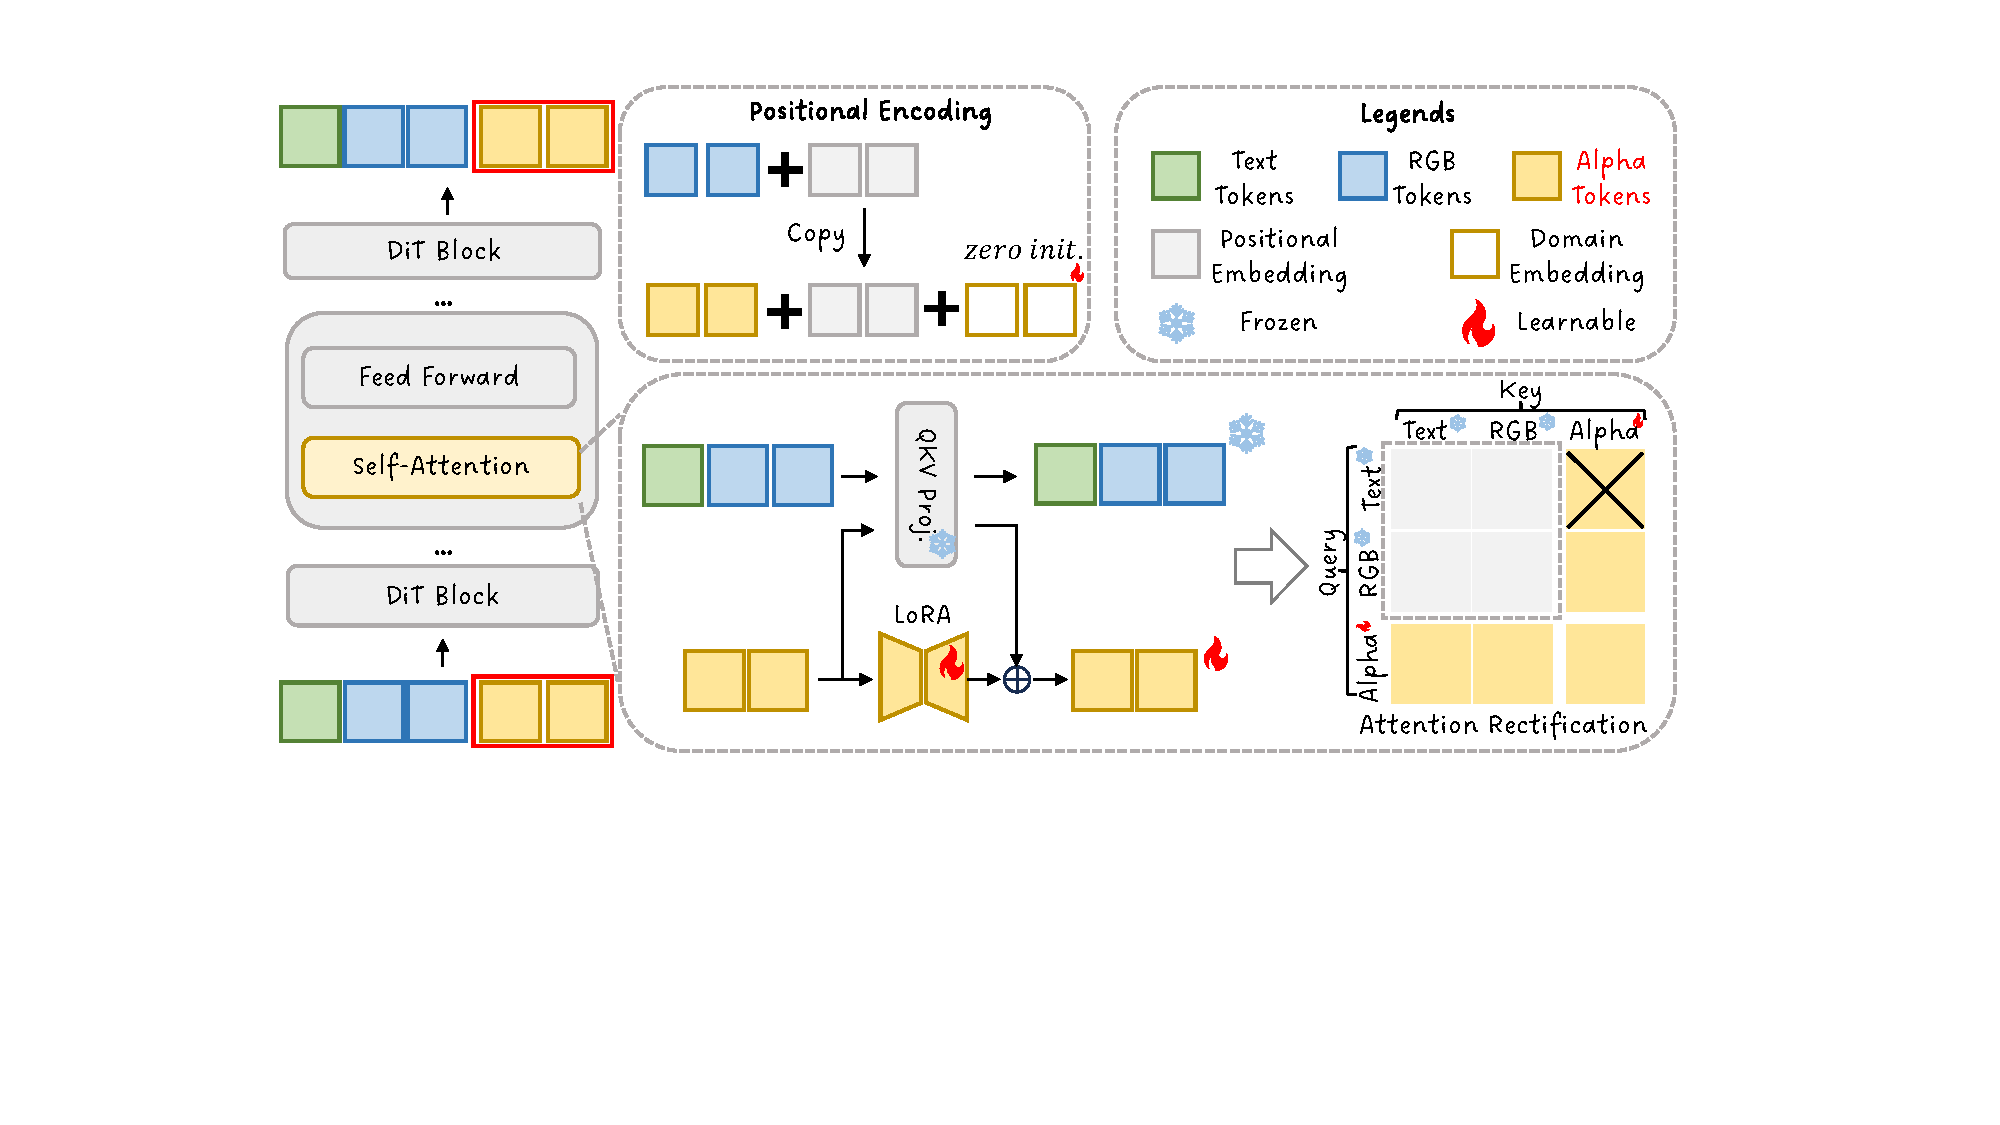
\includegraphics[width=1.0\linewidth]{figs/method-pipeline.pdf}
    \vspace{-0.2in}
    \caption{\textbf{Pipeline of TransPixar.} Our method is organized as follows: (1) \textbf{Left}: we extend the input of DiT to include new alpha tokens; (2) \textbf{Top Center}: we initialize alpha tokens with our positional encoding; (3) \textbf{Bottom Cente}r: we insert a partial LoRA and adjust attention computation during training and inference.}
    \label{fig-pipeline}
    \vspace{-0.1in}
\end{figure*}


% %-------------------------------------------------------------------------
\subsection{Preliminary}
We first introduce the open-sourced state-of-the-art DiT-based video generation models~\cite{yang2024cogvideox,genmo2024mochi}.
The core components of DiT-based video models are attention modules, and there are two primary distinctions between these models and previous approaches.
On one hand, unlike previous models that alternate between 1D temporal attention and 2D spatial attention~\cite{cerspense2023zeroscope, chen2023videocrafter1, chen2024videocrafter2, opensora}, current methods typically employ 3D spatio-temporal attention, allowing them to capture spatio-temporal dependencies more effectively.
On the other hand, instead of using cross-attention for text conditioning, these models concatenate text tokens \( \mathbf{x}_{\text{text}} \) with visual tokens \( \mathbf{x}_{\text{video}} \) into a single long sequence. 
The shape of video tokens and text tokens are \(B\times L\times D\) and \(B\times L_{\text{text}}\times D\), wher \(B\) equals to batch size, \(L_{\text{text}}\) equals to the length of text tokens, \(L\) equals to the length of video tokens and \(D\) equals to the latent dimension of transformer.
Full self-attention is then applied across the combined sequence:
\begin{equation}
\begin{aligned}
    &\text{Attention}(\mathbf{Q}, \mathbf{K}, \mathbf{V}) = \text{softmax}\left(\frac{\mathbf{Q}\mathbf{K}^T}{\sqrt{d_k}}\right)\mathbf{V}, \quad \text{where} \\
&\mathbf{Z : Z \in \{Q, K, V\}} \\&= [\mathbf{W}_{z : z \in \{q, k, v\}}(\mathbf{x}_{\text{text}}); \mathbf{f}_{z : z \in \{q, k, v\}}(\mathbf{x}_{\text{video}})]
\end{aligned}
\label{SA}
\end{equation}


Here \( \mathbf{W}_{t} \) (for \( t \in \{q, k, v\} \)) represents the projection matrixs in the transformer model, and \( \mathbf{f}_{t} \) (for \( t \in \{q, k, v\} \)) represents a combined operation that incorporates both the projection and positional encoding for visual tokens. 
There are two commonly used types of positional encoding. One is absolute positional encoding formulated as follows:
\begin{equation}
\begin{aligned}
\mathbf{f}_{z : z \in \{q, k, v\}}(\mathbf{x}_{\text{video}}) := \mathbf{W}_{z : z \in \{q, k, v\}}(\mathbf{x}_{\text{video}}^m + \mathbf{p}^m),
\end{aligned}
\label{PE}
\end{equation}
where \( \mathbf{p} \) is the positional embedding (e.g., a sinusoidal function) and \( m \) denotes the position of each RGB video token.
Another approach is the Rotary Position Embedding (RoPE)~\cite{su2024roformer}, often used by~\cite{yang2024cogvideox, genmo2024mochi}. 
This is expressed as
\begin{equation}
\begin{aligned}
\mathbf{f}_{z : z \in \{q, k\}}(\mathbf{x}_{\text{video}}) := \mathbf{W}_{z : z \in \{q, k\}}(\mathbf{x}_{\text{video}}^m) \circ e^{im\theta},
\end{aligned}
\label{RoPE}
\end{equation}
where \( m \) is the positional index, \( i \) is the imaginary unit for rotation, and \( \theta \) is the rotation angle.




% %-------------------------------------------------------------------------
\subsection{Our Approach} 
To jointly generate RGB and alpha videos, we adapt a pretrained RGB video generation model through several modifications. The whole pipeline is visualized in Fig.~\ref{fig-pipeline}.

Firstly, we double the sequence length of noisy input tokens to enable the model to generate videos of double length, from \( \mathbf{x}^{1:L}_{\text{video}} \) to \( \mathbf{x}^{1:2*L}_{\text{video}} \). 
Here, \( \mathbf{x}^{1:L}_{\text{video}} \) will be decoded into the RGB video, while \( \mathbf{x}^{L+1:2*L}_{\text{video}} \) will be decoded into the corresponding alpha video.
The Query(Q), Key(K), Value(V) representations are formulated as:
\begin{equation}
\begin{aligned}
&\mathbf{Z : Z \in \{Q, K, V\}} \\&= [\mathbf{W}_{z : z \in \{q, k, v\}}(\mathbf{x}_{\text{text}}); \mathbf{f}_{z : z \in \{q, k, v\}}(\mathbf{x}^{1:2*L}_{\text{video}})]
\end{aligned}
\end{equation}

In addition to sequence doubling, we explored increasing batch size or latent dimensions and splitting output into two domains; however, these approaches showed limited effectiveness under constrained datasets, which we discuss later.

Secondly, we modify the positional encoding function \( \mathbf{f}_{t : t \in \{q, k, v\}}(\cdot) \), as shown in Fig.~\ref{fig-pe}.
Instead of continuously numbering indices, we allow RGB and alpha tokens to share the same positional encoding. 
Taking absolute positional encoding as an example:
\begin{equation}
\begin{aligned}
&\mathbf{f}^*_{z : z \in \{q, k, v\}}(\mathbf{x}_{\text{video}}) \\:=
&\begin{cases}
\mathbf{W}_{z : z \in \{q, k, v\}}(\mathbf{x}_{\text{video}}^m + \mathbf{p}^m), & \text{if } m \leq L, \\
\mathbf{W}^*_{z : z \in \{q, k, v\}}(\mathbf{x}_{\text{video}}^m + \mathbf{p}^{m-L} + d), & \text{if } m > L.
\end{cases}
\label{eq:our_pe}
\end{aligned}
\end{equation}

Here we introduce a domain embedding \( d \), initialized to zero. We make it learnable to help the model adaptively differentiate between RGB (\(m\leq L\)) and alpha tokens (\(m>L \)). 
%
The motivation behind this design is we observe that with same postional encoding, even initializing with different noises, the tokens from two domains tend to generate same results. 
It minimizes spatial-temporal alignment challenges at the very beginning of training and thus accelerates convergence.

Next we propose a fine-tuning scheme using LoRA~\cite{hu2021lora}, in which the LoRA layer is applied only to alpha domain tokens:
\begin{equation}
\begin{aligned}
&\mathbf{W}^*_{z : z \in \{q, k, v\}}(\mathbf{x}_{\text{video}}^m + \mathbf{p}^{m-L} + d)\\=
&\ \mathbf{W}_{z : z \in \{q, k, v\}}(\mathbf{x}_{\text{video}}^m + \mathbf{p}^{m-L} + d)
\\
+\ &\gamma\cdot \text{LoRA}(\mathbf{x}_{\text{video}}^m + \mathbf{p}^{m-L} + d), \quad \text{if } m > L,
\label{eq:our_lora}
\end{aligned}
\end{equation}
where \( \gamma \) controls the residual strength. 
Additionally, we design an attention mask to block unwanted attention computation. 
Given a text-video token sequence length \( L_\text{text} + 2L \), where \( L_\text{text} \) represents text token length, the mask is defined as:
\begin{equation}
\mathbf{M}^*_{mn} = 
\begin{cases} 
-\infty, & \text{if } m \leq L_\text{text} \ \text{and} \ \, n > L_\text{text} + L, \\
0, & \text{otherwise}.
\end{cases}
\label{eq:attn_mask}
\end{equation}

Combining these modifications, inference with our method is expressed as:
\begin{equation}
\begin{aligned}
    &\text{Attention}(\mathbf{Q}, \mathbf{K}, \mathbf{V}) = \text{softmax}\left(\frac{\mathbf{Q}\mathbf{K}^T}{\sqrt{d_k}}+\mathbf{M}^*\right)\mathbf{V}, \quad \text{where} \\
&\mathbf{Z : Z \in \{Q, K, V\}} \\&= [\mathbf{W}_{z : z \in \{q, k, v\}}(\mathbf{x}_{\text{text}}); \mathbf{f}^*_{z : z \in \{q, k, v\}}(\mathbf{x}_{\text{video}})]
\end{aligned}
\label{eq:our_method}
\end{equation}

Training is carried out using flow matching~\cite{liu2022flow} or a traditional diffusion process~\cite{ho2020denoising}.


\begin{figure}[t]
    \centering
    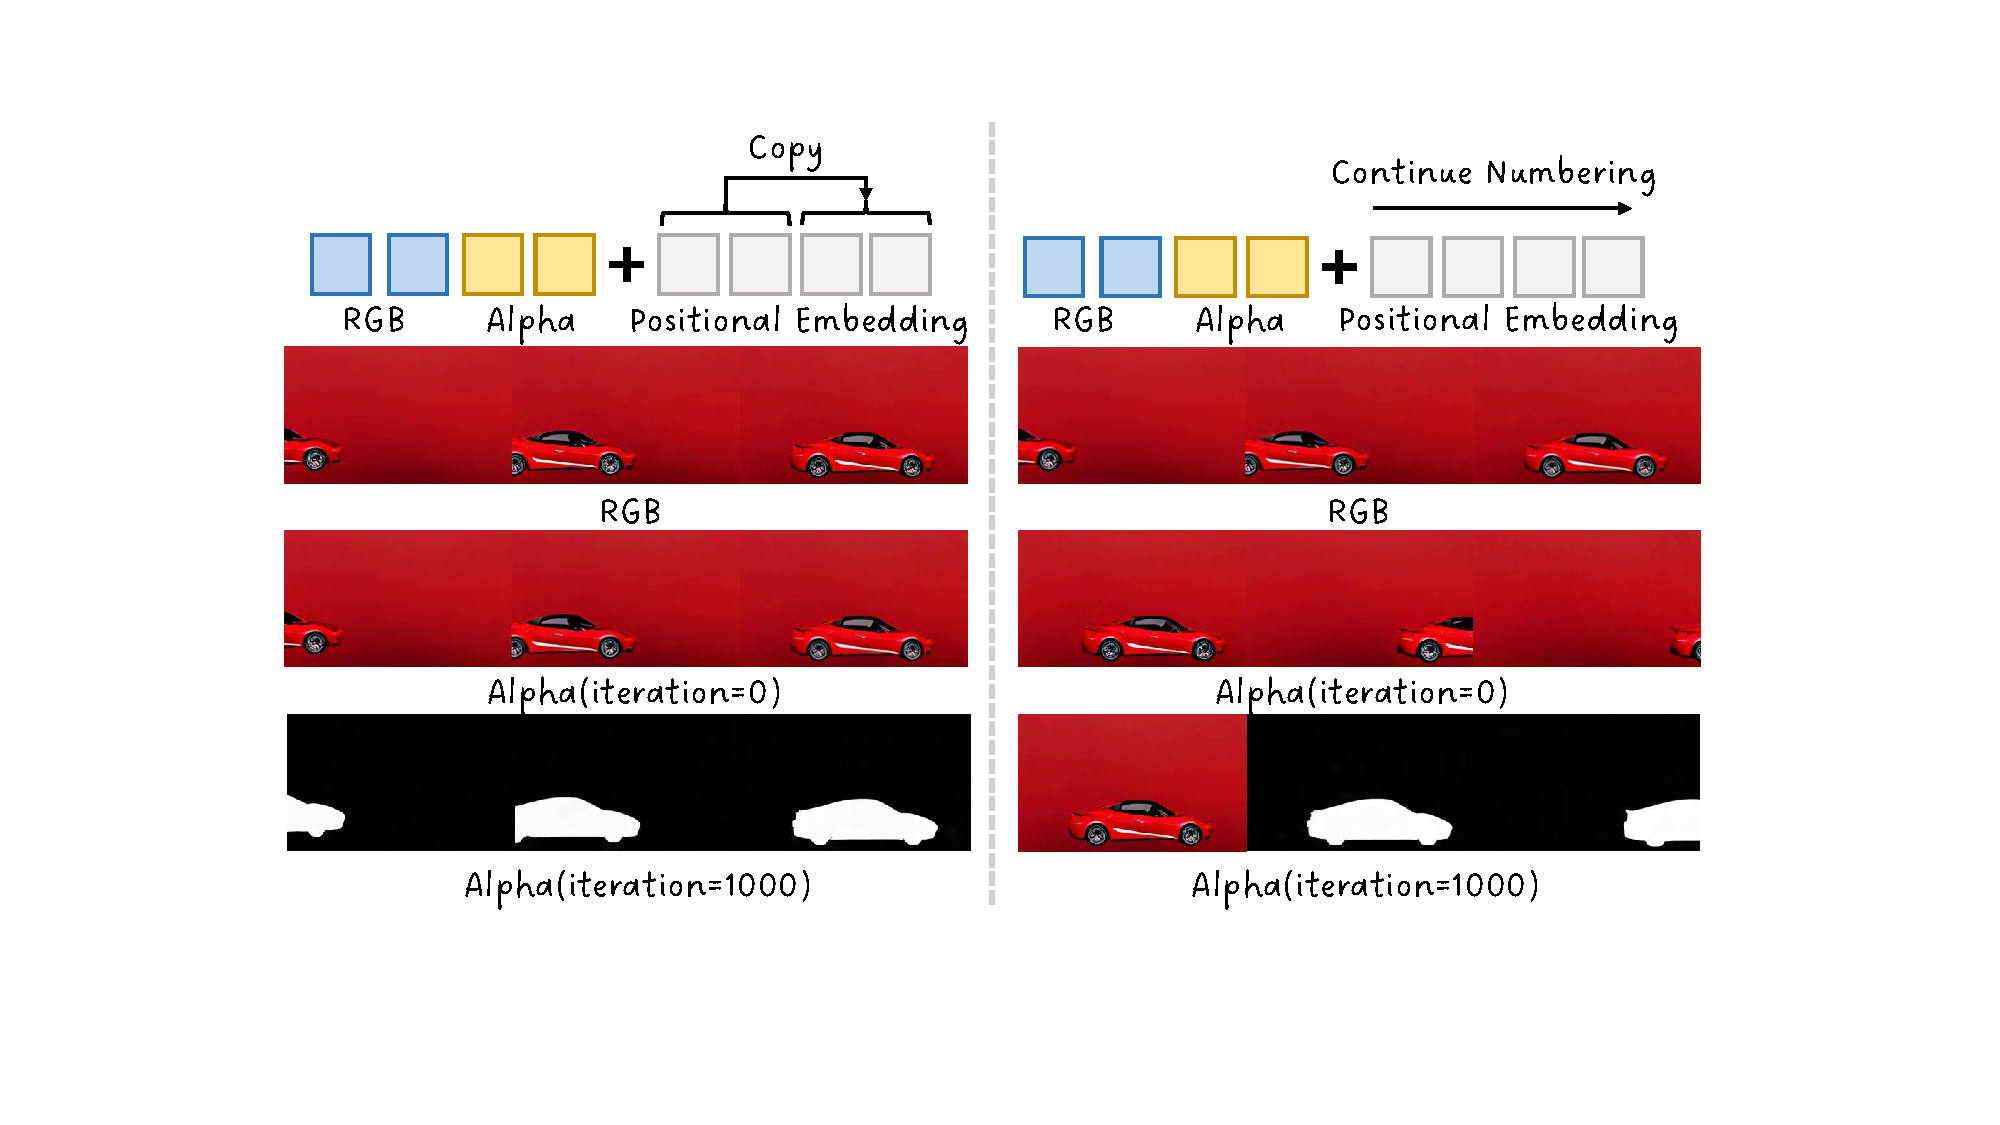
\includegraphics[width=1.0\linewidth]{figs/method-pe_init.pdf}
    \vspace{-0.2in}
    \caption{\textbf{Positional Encoding Design for RGBA Generation.} Assigning alpha tokens the same positional encoding as RGB yields similar results, resulting in faster convergence after 1000 iterations compared to standard encoding strategies.}
    \label{fig-pe}
    \vspace{-0.1in}
\end{figure}

% %-------------------------------------------------------------------------
\subsection{Analysis}
% % given our goal is 最大程度地继承 pretrain video model的能力,让它能生成的东西超越已有的RGBA训练集,
% 在目前我们使用的3d full attention DiT的video generation model的框架下,最重要的计算是attention mechanism,因此我们进一步对该过程进行分析:
% The attention matrix, \(\mathbf{Q}\mathbf{K}^T\), now has dimensions \((L_\text{text} + 2*L) \times (L_\text{text} + 2*L)\), which we simplify by organizing it into a 3x3 grouped attention matrix—\textbf{Text-attend-to-RGB}, \textbf{RGB-attend-to-Text}, and so forth, as illustrated in Fig.~\ref{fig-pipeline}. Then we procceed to analyze them:

% \noindent{\textbf{Text-Attend-to-RGB} and \textbf{RGB-Attend-to-Text}}.
% Given this matrix, we are supposed to preserve as much of the computation in the upper-left 2x2 section as possible so that we can preserve the RGB generation potential. 

% These represent the upper-left 2x2 section in \(\mathbf{Q}\mathbf{K}^T\) and 是RGB original generation model有且仅有的计算过程,如果我们能保证这部分计算不受影响,we can replicate the original RGB generation performance. 
% Therefore, we limited the scope of LoRA's influence, as defined in Equation~\eqref{eq:our_lora}, we retain the original QKV values for both text and RGB tokens, maintaining the pretrained model’s behavior in these domains.

% Besides the partial lora, the introduction of alpha tokens make the text and RGB tokens need to act as key and interact with alpha tokens as query, which will also 改变这个2x2 attention matrix的计算结果。
% Therefore, we proceed to analyze two additional attention computations that affect RGB generation shown in Fig.~\ref{fig-attn}:


% \noindent{\textbf{Text-Attend-to-Alpha}}: We find this attention is detrimental to the generation quality. 
% Since the model is originally trained with text and RGB data, introducing attention from text to alpha causes interference due to the domain gap between alpha and RGB. 
% Specifically, alpha modality provide only contour information and lack the rich texture, color, and semantic details associated with text prompt, thereby degrading generation quality. 
% To mitigate this, we design the attention mask (Equation~\eqref{eq:attn_mask}) that blocks this computation.

% \noindent{\textbf{RGB-Attend-to-Alpha}}: In contrast, we identify \textbf{RGB-to-Alpha} as essential for successful joint generation. 
% This attention allows the model to refine RGB tokens by considering alpha information, facilitating alignment between generated RGB and alpha channels. 
% This refinement process is a critical component missing in prior generation-then-prediction pipelines, which lack a feedback mechanism for RGB refinement based on alpha guidance.
Given our goal of maximizing the inherited capabilities of the pretrained video model, enabling it to generate beyond the existing RGBA training set, we analyze the most critical component within our current 3D full attention DiT video generation model: the attention mechanism.
%
The attention matrix, \(\mathbf{Q}\mathbf{K}^T\), has dimensions \((L_\text{text} + 2*L) \times (L_\text{text} + 2*L)\), which we simplify by organizing it into a 3x3 grouped attention matrix—including \textbf{Text-attend-to-RGB}, \textbf{RGB-attend-to-Text}, and so forth, as illustrated in Fig.~\ref{fig-pipeline}. %We then analyze these components:

\vspace{0.5em}
\noindent\textbf{Text-Attend-to-RGB and RGB-Attend-to-Text}. These represent the upper-left 2x2 section of  and are computations that exist solely in the original RGB generation model. If we ensure that this part of the computation remains unaffected, we can replicate the original RGB generation performance. Therefore, we limit the scope of LoRA's influence, as defined in Eq.~\eqref{eq:attn_mask}, by retaining the original QKV values for both text and RGB tokens, thus preserving the pretrained model’s behavior in these domains.

Besides the partial LoRA, the added alpha tokens requires the text and RGB tokens to also act as queries and interact with the alpha tokens as keys, which alters the computation in this 2x2 attention matrix. 
Therefore, we further analyze two additional attention computations that impact RGB generation, as shown in Fig.~\ref{fig-attn}.

\vspace{0.5em}
\noindent\textbf{Text-Attend-to-Alpha.} We find that this attention is detrimental to the generation quality. Since the model was originally trained with text and RGB data, introducing attention from text to alpha causes interference due to the domain gap between alpha and RGB. Specifically, the alpha modality provides only contour information and lacks the rich texture, color, and semantic details associated with the text prompt, thereby degrading generation quality. To mitigate this, we design the attention mask (Eq.~\eqref{eq:attn_mask}) that blocks this computation.

\vspace{0.5em}
\noindent\textbf{RGB-Attend-to-Alpha.} In contrast, we identify \textbf{RGB-to-Alpha} as essential for successful joint generation. This attention allows the model to refine RGB tokens by considering alpha information, facilitating alignment between generated RGB and alpha channels. This refinement process is a critical component missing in previous generation-then-prediction pipelines, which lacked a feedback mechanism for RGB refinement based on alpha guidance.


\begin{figure}[t]
    \centering
    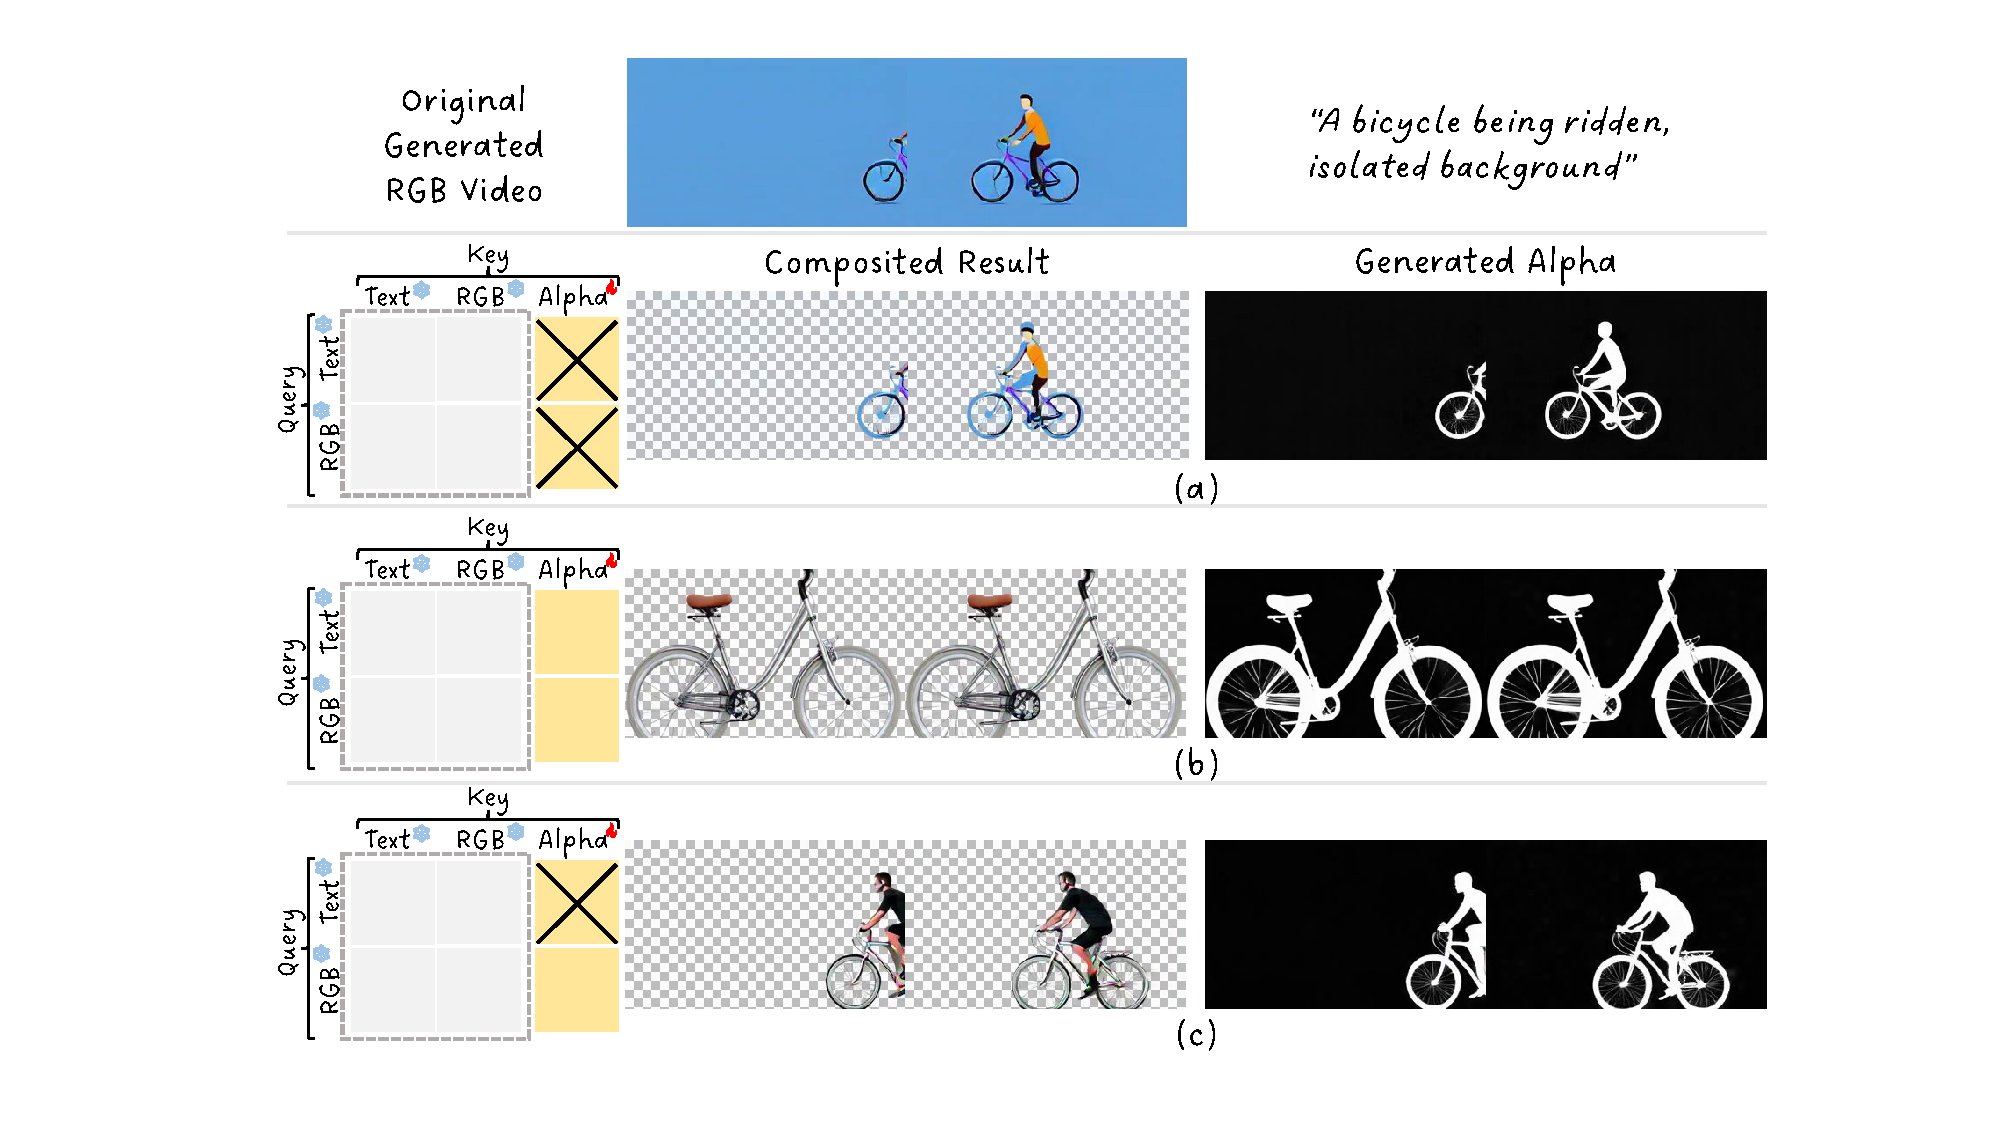
\includegraphics[width=1.0\linewidth]{figs/method-attn.pdf}
    \vspace{-0.2in}
    \caption{\textbf{Attention Rectification.} (a) Eliminating all attention from alpha as a key preserves 100\% RGB generation but leads to poor alignment. (b) Retaining all attention significantly degrades quality, causing a lack of motion in bicycles. (c) Our method achieves an effective balance.
    }
    \label{fig-attn}
    \vspace{-0.1in}
\end{figure}



